% This is LLNCS.DEM the demonstration file of
% the LaTeX macro package from Springer-Verlag
% for Lecture Notes in Computer Science,
% version 2.4 for LaTeX2e as of 16. April 2010
%
\RequirePackage{amsmath,amssymb}
\documentclass{llncs}
%
\usepackage{stmaryrd}
\usepackage{wasysym}
\usepackage{makeidx}  % allows for indexgeneration
\usepackage{mathpartir} % inference rules
\usepackage{extarrows}
\usepackage{graphicx}
\usepackage{url}

% !TEX root = editor-tfp16.tex

% HTyp and HExp
\newcommand{\hcomplete}[1]{#1~\mathsf{complete}}

% HTyp
\newcommand{\htau}{\dot{\tau}}
\newcommand{\tarr}[2]{#1 \rightarrow #2}
\newcommand{\tnum}{\texttt{num}}
\newcommand{\tehole}{\llparenthesis\rrparenthesis}

\newcommand{\tcompat}[2]{#1 \sim #2}

% HExp
\newcommand{\hexp}{\dot{e}}
\newcommand{\hlam}[3]{\lambda #1{:}#2.#3}
\newcommand{\hap}[2]{#1(#2)}
\newcommand{\hnum}[1]{\underline{#1}}
\newcommand{\hadd}[2]{#1 + #2}
\newcommand{\hehole}{\llparenthesis\rrparenthesis}
\newcommand{\hhole}[1]{\llparenthesis#1\rrparenthesis}

\newcommand{\hGamma}{\dot{\Gamma}}
\newcommand{\domof}[1]{\text{dom}(#1)}
\newcommand{\hsyn}[3]{#1 \vdash #2 \Rightarrow #3}
\newcommand{\hana}[3]{#1 \vdash #2 \Leftarrow #3}

% ZTyp and ZExp
\newcommand{\zlsel}[1]{{\bowtie}{#1}}
\newcommand{\zrsel}[1]{{#1}{\bowtie}}
\newcommand{\zwsel}[1]{{\triangleright}{#1}{\triangleleft}}

\newcommand{\removeSel}[1]{#1^{\diamond}}

% ZTyp
\newcommand{\ztau}{\hat{\tau}}

% ZExp
\newcommand{\zexp}{\hat{e}}

% Direction
\newcommand{\dParent}{\mathtt{parent}}
\newcommand{\dChild}{\mathtt{firstChild}}
\newcommand{\dNext}{\mathtt{nextSib}}
\newcommand{\dPrev}{\mathtt{prevSib}}

% Action
\newcommand{\aMove}[1]{\mathtt{move}~#1}
	\newcommand{\zrightmost}[1]{\mathsf{rightmost}(#1)}
	\newcommand{\zleftmost}[1]{\mathsf{leftmost}(#1)}
\newcommand{\aSelect}[1]{\mathtt{sel}~#1}
\newcommand{\aDel}{\mathtt{del}}
\newcommand{\aReplace}[1]{\mathtt{replace}~#1}
\newcommand{\aConstruct}[1]{\mathtt{construct}~#1}
\newcommand{\aFinish}{\mathtt{finish}}

\newcommand{\performAna}[5]{#1 \vdash #2 \Leftarrow #3 \xlongrightarrow{#4} #5}
\newcommand{\performSyn}[5]{#1 \vdash #2 \Rightarrow #3 \xlongrightarrow{#4} #5}
\newcommand{\performTyp}[3]{#1 \xlongrightarrow{#2} #3}

\newcommand{\performMove}[3]{#1 \xlongrightarrow{#2} #3}
\newcommand{\performDel}[2]{#1 \xlongrightarrow{\aDel} #2}

% Form
\newcommand{\farr}{\mathtt{arr}}
\newcommand{\fnum}{\mathtt{num}}

\newcommand{\fasc}{\mathtt{asc}}
\newcommand{\fvar}[1]{\mathtt{var}~#1}
\newcommand{\flam}[1]{\mathtt{lam}~#1}
\newcommand{\fap}{\mathtt{ap}}
\newcommand{\fnumlit}[1]{\mathtt{numlit}~#1}
\newcommand{\fplus}{\mathtt{plus}}
\newcommand{\fhole}{\mathtt{hole}}

%
\begin{document}

%
\frontmatter          % for the preliminaries
%
%\pagestyle{headings}  % switches on printing of running heads
%\addtocmark{Hamiltonian Mechanics} % additional mark in the TOC
%
% \chapter*{Preface}
% %
% This textbook is intended for use by students of physics, physical
% chemistry, and theoretical chemistry. The reader is presumed to have a
% basic knowledge of atomic and quantum physics at the level provided, for
% example, by the first few chapters in our book {\it The Physics of Atoms
% and Quanta}. The student of physics will find here material which should
% be included in the basic education of every physicist. This book should
% furthermore allow students to acquire an appreciation of the breadth and
% variety within the field of molecular physics and its future as a
% fascinating area of research.

% For the student of chemistry, the concepts introduced in this book will
% provide a theoretical framework for that entire field of study. With the
% help of these concepts, it is at least in principle possible to reduce
% the enormous body of empirical chemical knowledge to a few basic
% principles: those of quantum mechanics. In addition, modern physical
% methods whose fundamentals are introduced here are becoming increasingly
% important in chemistry and now represent indispensable tools for the
% chemist. As examples, we might mention the structural analysis of
% complex organic compounds, spectroscopic investigation of very rapid
% reaction processes or, as a practical application, the remote detection
% of pollutants in the air.

% \vspace{1cm}
% \begin{flushright}\noindent
% April 1995\hfill Walter Olthoff\\
% Program Chair\\
% ECOOP'95
% \end{flushright}
% %
% \chapter*{Organization}
% ECOOP'95 is organized by the department of Computer Science, Univeristy
% of \AA rhus and AITO (association Internationa pour les Technologie
% Object) in cooperation with ACM/SIGPLAN.
% %
% \section*{Executive Commitee}
% \begin{tabular}{@{}p{5cm}@{}p{7.2cm}@{}}
% Conference Chair:&Ole Lehrmann Madsen (\AA rhus University, DK)\\
% Program Chair:   &Walter Olthoff (DFKI GmbH, Germany)\\
% Organizing Chair:&J\o rgen Lindskov Knudsen (\AA rhus University, DK)\\
% Tutorials:&Birger M\o ller-Pedersen\hfil\break
% (Norwegian Computing Center, Norway)\\
% Workshops:&Eric Jul (University of Kopenhagen, Denmark)\\
% Panels:&Boris Magnusson (Lund University, Sweden)\\
% Exhibition:&Elmer Sandvad (\AA rhus University, DK)\\
% Demonstrations:&Kurt N\o rdmark (\AA rhus University, DK)
% \end{tabular}
% %
% \section*{Program Commitee}
% \begin{tabular}{@{}p{5cm}@{}p{7.2cm}@{}}
% Conference Chair:&Ole Lehrmann Madsen (\AA rhus University, DK)\\
% Program Chair:   &Walter Olthoff (DFKI GmbH, Germany)\\
% Organizing Chair:&J\o rgen Lindskov Knudsen (\AA rhus University, DK)\\
% Tutorials:&Birger M\o ller-Pedersen\hfil\break
% (Norwegian Computing Center, Norway)\\
% Workshops:&Eric Jul (University of Kopenhagen, Denmark)\\
% Panels:&Boris Magnusson (Lund University, Sweden)\\
% Exhibition:&Elmer Sandvad (\AA rhus University, DK)\\
% Demonstrations:&Kurt N\o rdmark (\AA rhus University, DK)
% \end{tabular}
% %
% \begin{multicols}{3}[\section*{Referees}]
% V.~Andreev\\
% B\"arwolff\\
% E.~Barrelet\\
% H.P.~Beck\\
% G.~Bernardi\\
% E.~Binder\\
% P.C.~Bosetti\\
% Braunschweig\\
% F.W.~B\"usser\\
% T.~Carli\\
% A.B.~Clegg\\
% G.~Cozzika\\
% S.~Dagoret\\
% Del~Buono\\
% P.~Dingus\\
% H.~Duhm\\
% J.~Ebert\\
% S.~Eichenberger\\
% R.J.~Ellison\\
% Feltesse\\
% W.~Flauger\\
% A.~Fomenko\\
% G.~Franke\\
% J.~Garvey\\
% M.~Gennis\\
% L.~Goerlich\\
% P.~Goritchev\\
% H.~Greif\\
% E.M.~Hanlon\\
% R.~Haydar\\
% R.C.W.~Henderso\\
% P.~Hill\\
% H.~Hufnagel\\
% A.~Jacholkowska\\
% Johannsen\\
% S.~Kasarian\\
% I.R.~Kenyon\\
% C.~Kleinwort\\
% T.~K\"ohler\\
% S.D.~Kolya\\
% P.~Kostka\\
% U.~Kr\"uger\\
% J.~Kurzh\"ofer\\
% M.P.J.~Landon\\
% A.~Lebedev\\
% Ch.~Ley\\
% F.~Linsel\\
% H.~Lohmand\\
% Martin\\
% S.~Masson\\
% K.~Meier\\
% C.A.~Meyer\\
% S.~Mikocki\\
% J.V.~Morris\\
% B.~Naroska\\
% Nguyen\\
% U.~Obrock\\
% G.D.~Patel\\
% Ch.~Pichler\\
% S.~Prell\\
% F.~Raupach\\
% V.~Riech\\
% P.~Robmann\\
% N.~Sahlmann\\
% P.~Schleper\\
% Sch\"oning\\
% B.~Schwab\\
% A.~Semenov\\
% G.~Siegmon\\
% J.R.~Smith\\
% M.~Steenbock\\
% U.~Straumann\\
% C.~Thiebaux\\
% P.~Van~Esch\\
% from Yerevan Ph\\
% L.R.~West\\
% G.-G.~Winter\\
% T.P.~Yiou\\
% M.~Zimmer\end{multicols}
% %
% \section*{Sponsoring Institutions}
% %
% Bernauer-Budiman Inc., Reading, Mass.\\
% The Hofmann-International Company, San Louis Obispo, Cal.\\
% Kramer Industries, Heidelberg, Germany
% %
% \tableofcontents
% %
\mainmatter              % start of the contributions
%
\title{Hazelnut: A Minimal Bidirectionally Typed Structure Editor}
%
%\titlerunning{Hamiltonian Mechanics}  % abbreviated title (for running head)
%                                     also used for the TOC unless
%                                     \toctitle is used
%
\author{Cyrus Omar\inst{1}$^\dagger$ \and Michael Hilton\inst{2}$^\dagger$ \and
Ian Voysey\inst{1}$^\dagger$ \and \\Jonathan Aldrich\inst{1} \and Matthew A. Hammer\inst{3}}
%
\authorrunning{Omar et al.} % abbreviated author list (for running head)
%
%%%% list of authors for the TOC (use if author list has to be modified)
%\tocauthor{Ivar Ekeland, Roger Temam, Jeffrey Dean, David Grove,
%Craig Chambers, Kim B. Bruce, and Elisa Bertino}
%
\institute{Carnegie Mellon University
%\email{comar@cs.cmu.edu}\\
%\texttt{http://www.cs.cmu.edu/\homedir comar/}
\and
Oregon State University
%\email{hiltonm@eecs.oregonstate.edu}\\
\and
University of Colorado Boulder
%\email{Matthew.Hammer@colorado.edu}
\\
{}$^\dagger$~{Student Author}
}

\maketitle              % typeset the title of the contribution
\begin{abstract}
Programs (and proofs) are rich inductive structures, but  programmers typically construct and manipulate them only indirectly, through flat textual representations. This indirection  comes at a cost -- programmers must comprehend the various subtleties of textual syntax, and it can take several text editor actions to make a single structural change. During these sequences of text editor actions, code highlighters and various other assistive tools are asked to reason about malformed program text, complicating their design.
%Unfortunately, this fact is somewhat obscure because  programmers typically construct and interact with  programs only indirectly, using a text editor composed with a parser.
%There are some benefits to this approach, to be sure, but the structural mismatch between programs and text  also imposes a cognitive burden.
%For example, the primitive edit actions available in a text editor (e.g. inserting or deleting a character or word)  do not always correspond to  sensible structural transformations.
%Indeed, most structural  transformations require performing many primitive edit actions.

\emph{Structure editors} promise to alleviate these burdens by exposing only edit actions that  correspond to  sensible structural  transformations.
Existing designs for structure editors, however, are complex and somewhat \emph{ad hoc}.
Our aim in this paper is to report on our ongoing efforts to develop Hazelnut, a minimal type-theoretic structure editor.
Hazelnut is based on  a standard bidirectionally typed lambda calculus. We extend this calculus with
1) \emph{holes} (which mark portions of the program that remain under construction);
%, which are identified by variables tracked in a separate linear \emph{hole context}
2) a \emph{cursor model}; and 3) an \emph{action model}. Programs with holes have a well-defined static semantics in Hazelnut, and the action model is defined such that every performable action is both syntactically sensible (by construction) and semantically sensible (i.e. we can establish an \emph{action sensibility} theorem.)
We conclude by outlining our vision of a full-scale programming system grown ``from the ground up'' around the same fundamental concepts as Hazelnut.

%\keywords{computational geometry, graph theory, Hamilton cycles}
\end{abstract}
%
\section{Introduction}
%
Programs (and, by the Curry-Howard correspondence, proofs) are rich inductive structures. This fact is well understood amongst researchers and experienced programmers, but still somewhat  obscure amongst programmers at large because programmers normally construct and interact with  programs only indirectly, e.g. using a text editor composed with a parser.

There are some benefits to this approach, to be sure, but the structural mismatch between programs and their textual representations  also imposes various burdens.
For example, the primitive edit actions available in a text editor (e.g. inserting or deleting a character or word)  do not always correspond to  sensible structural transformations.


\paragraph{Example: Structured Interaction in Hazelnut.}
%
Figure~\ref{fig:first-example} gives an example of the Hazelnut user
programming the identity function over numbers, then applying this
function to an argument, the number literal~3.
%
Lines 1--10 consist of the user interactively constructing the
identity function.
%
After the break, lines 11--15 consist of the user editing this program
so that it consists of a function application (of the first program)
to the literal argument~3.

Line~1 begins with the initial, empty state: The H-Expression and
Z-Expression are each empty; they differ only in that the Z-Expression
focuses on the hole of the H-Expression.
%
The syntax~$\zwsel{\cdot}$ indicates the current user focus, which
determines where actions transform the expressions.
%
The third column~(\textbf{Next Action}) lists the first user action:
Constructing a lambda abstraction using variable~$x$.
%
The final column~(\textbf{Semantics}) indicates the semantic rule for
this action, Rule (20e), which gives general semantics for introducing
lambda terms into holes.
%
In Section~\ref{sec:?}, we list this rule, and the other rules used in
this final column. In total, these rules give a formal semantics to
the user actions, which relate each line's Z-Expression to the
Z-Expression on the subsequent line.

In addition to introducing the lambda term, and its variable, the
first user action~$\aConstruct{\flam{x}}$ also introduces a type
ascription for this function, as an arrow type, with holes for the
type of its domain and codomain.
%
The actions for Lines~2--5 consist of the user filling these holes
with the basetype $\tnum{}$.
%
To do so, the user constructs the type constructor twice (Lines 2 and
4), and navigates between the holes with a move action (Line~3).
%
Generally, the move action~$\dNext$ moves the focus from one
sub-structure to the next sibling sub-structure of the (common) parent
structure; in this case, it moves from the domain type of the arrow
type to the codomain of the arrow type.
%

\begin{figure}[t]
\[
\begin{array}{|c||c|c||l|l|}
\hline
\# & \textbf{H-Expression} & \textbf{Z-Expression} & \textbf{Next Action} & \textbf{Semantics}
\\
\hline
1 &
\hhole{} &
\zwsel{\hhole{}}
&
\aConstruct{\flam{x}} & \refrule{20e}
\\ 2 &
\hlam{x}{\hhole{}} : \tarr{\hhole{}}{\hhole{}} &
\hlam{x}{\hhole{}} : \tarr{\zwsel{\hhole{}}}{\hhole{}}
&
\aConstruct{\fnum{}} & \refrule{19b}
\\ 3 &
\hlam{x}{\hhole{}} : \tarr{\tnum{}}{\hhole{}} &
\hlam{x}{\hhole{}} : \tarr{\zwsel{\tnum{}}}{\hhole{}}
&
\aMove{\dNext{}} & \refrule{15d}
\\ 4 &
&
\hlam{x}{\hhole{}} : \tarr{\tnum}{\zwsel{\hhole{}}}
&
\aConstruct{\fnum{}} & \refrule{19b}
\\ 5 &
\hlam{x}{\hhole{}} : \tarr{\tnum{}}{\tnum{}} &
\hlam{x}{\hhole{}} : \tarr{\tnum{}}{\zwsel{\tnum{}}}
&
\aMove{\dParent{}} & \refrule{15b}
\\ 6 &
&
\hlam{x}{\hhole{}} : \zwsel{\tarr{\tnum{}}{\tnum{}}}
&
\aMove{\dPrev{}} & \refrule{15e}
\\ 7 &
&
\zwsel{\hlam{x}{\hhole{}}} : \tarr{\tnum{}}{\tnum{}}
&
\aMove{\dChild{}} & \refrule{15a}
\\ 8 &
&
\hlam{x}{\zwsel{\hhole{}}} : \tarr{\tnum{}}{\tnum{}}
&
\aConstruct{\fvar{x}} & \refrule{20c}
%\\ 9 &
%\hlam{x}{\hhole{x}} : \tarr{\tnum{}}{\tnum{}}
%&
%\hlam{x}{\zwsel{\hhole{x}}} : \tarr{\tnum{}}{\tnum{}}
%&
%\aFinish{} & \refrule{21a}
\\ 10 &
\hlam{x}{{x}} : \tarr{\tnum{}}{\tnum{}}
&
\hlam{x}{\zwsel{{x}}} : \tarr{\tnum{}}{\tnum{}}
&
\quad\textrm{---{}---}
&
\quad\textrm{---{}---}
\\
\hline
\hline
11 &
\hhole{\textrm{id}} : \tnum{} &
\hhole{\zwsel{{\textrm{id}}}} : \tnum{}
&
\aConstruct{\fap{}} & ?
\\
12 &
\hhole{\hap{{{\textrm{id}}}}{{\hhole{}}}} : \tnum{}
&
\hhole{\hap{{{\textrm{id}}}}{\zwsel{\hhole{}}}} : \tnum{}
&
\aConstruct{\fnumlit{3}} & ?
\\
13 &
\hhole{\hap{{{\textrm{id}}}}{{\hnum{3}}}} : \tnum{}
&
\hhole{\hap{{{\textrm{id}}}}{\zwsel{\hnum{3}}}} : \tnum{}
&
\aMove{\dParent{}} & ?
\\
14 &
%\hhole{\hap{{{\textrm{id}}}}{{\hnum{3}}}} : \tnum{}
&
\hhole{\zwsel{\hap{{{\textrm{id}}}}{{\hnum{3}}}}} : \tnum{}
&
\aMove{\dParent{}} & ?
\\
15 &
%\hhole{\hap{{{\textrm{id}}}}{{\hnum{3}}}} : \tnum{}
&
\zwsel{\hhole{{\hap{{{\textrm{id}}}}{{\hnum{3}}}}}} : \tnum{}
&
\aMove{\dParent{}} & ?
\\
16 &
{\hap{{{\textrm{id}}}}{{\hnum{3}}}} : \tnum{}
&
\zwsel{{{\hap{{{\textrm{id}}}}{{\hnum{3}}}}}} : \tnum{}
&
\aFinish & ?
\\
\hline

%% 11 &
%% {\textrm{id}} : \tarr{\tnum{}}{\tnum{}}
%% &
%% \hlam{x}{\zwsel{{x}}} : \tarr{\tnum{}}{\tnum{}}
%% &
%% \aMove{\dParent{}} & ?
%% \\ 12 &
%% %{\textrm{id}} : \tarr{\tnum{}}{\tnum{}}
%% &
%% \zwsel{\hlam{x}{{{x}}}} : \tarr{\tnum{}}{\tnum{}}
%% &
%% \aMove{\dParent{}} & \refrule{15b}
%% \\ 13 &
%% %{\textrm{id}} : \tarr{\tnum{}}{\tnum{}}
%% &
%% \zwsel{\hlam{x}{{{x}}} : \tarr{\tnum{}}{\tnum{}}}
%% &
%% \aConstruct{\fap{}} & \refrule{20h}
%% \\ 14 &
%% \hapP{{\textrm{id}} : \tarr{\tnum{}}{\tnum{}}}{\hhole{}}
%% &
%% \hapP{{\textrm{id}} : \tarr{\tnum{}}{\tnum{}}}{\zwsel{\hhole{}}}
%% &
%% \aConstruct{\fnumlit{3}} & \refrule{20l}
%% \\ 15 &
%% %\hapP{{\textrm{id}} : \tarr{\tnum{}}{\tnum{}}}{\hhole{3}}
%% %&
%% %\hapP{{\textrm{id}} : \tarr{\tnum{}}{\tnum{}}}{\zwsel{\hhole{3}}}
%% %&
%% %\aFinish{} & ?
%% %\\
%% \hapP{{\textrm{id}} : \tarr{\tnum{}}{\tnum{}}}{{\hnum{3}}}
%% &
%% \hapP{{\textrm{id}} : \tarr{\tnum{}}{\tnum{}}}{\zwsel{{\hnum{3}}}}
%% &
%% \quad\textrm{---{}---}
%% &
%% \quad\textrm{---{}---}
%% \\
%% \hline
\end{array}
\]
\caption{Example of interactively constructing identity function in Hazelnut (Lines~1--10).
  Afterward, the user applies this function to an argument~(Lines 11--15).}
\label{fig:first-example}
\end{figure}

\section{Hazelnut}
Hazelnut is based on the simply-typed lambda calculus extended with a single base type, $\tnum$. Its major constituents are:
\begin{itemize}
\item \textbf{H-types} and \textbf{H-expressions} (Sec. \ref{sec:holes}), which are terms with \emph{holes}. Holes mark subterms that are ``under construction.'' H-types classify H-expressions according to a {bidirectionally typed} static semantics.
\item \textbf{Z-types} and \textbf{Z-expressions} (Sec. \ref{sec:cursors}), which superimpose a single \emph{cursor} onto H-types and H-expressions (using the \emph{zipper pattern}.)
\item \textbf{Actions} (Sec. \ref{sec:actions}), which move the cursor or modify the subterm marked by the cursor.

Whenever an action is performed on a well-typed expression, it produces another well-typed expression in a \emph{sensible} manner -- we define \emph{sensibility} in Sec. \ref{sec:actions}.
\end{itemize}

\subsection{Holes}\label{sec:holes}
\begin{figure}
$\arraycolsep=4pt\begin{array}{lllllll}
\mathsf{HTyp} & \tau,\htau & ::= &
  \tarr{\htau}{\htau} ~\vert~
  \tnum ~\vert~
  \tehole\\
\mathsf{HExp} & e,\hexp & ::= &
  \hexp : \htau ~\vert~
  x ~\vert~
  \hlam{x}{\hexp} ~\vert~
  \hap{\hexp}{\hexp} ~\vert~
  \hnum{n} ~\vert~
  \hadd{\hexp}{\hexp} ~\vert~
  \hehole ~\vert~
  \hhole{\hexp}
\end{array}$
%\textbf{Sort} & & & \textbf{Operational Form} & \textbf{Stylized Form} & \textbf{Description}\\
\caption{Syntax of H-types and H-expressions. Metavariable $x$ ranges over variables and $n$ ranges over numerals.}
\label{fig:hexp-syntax}
\end{figure}

The syntax of H-types and H-expressions is given in Figure \ref{fig:hexp-syntax}. Most forms correspond directly to those of the simply-typed lambda calculus extended with type $\tnum$. The number expression corresponding to the number $n$ is drawn $\hnum{n}$, and for simplicity, we define only a single arithmetic operation, $\hadd{\hexp}{\hexp}$.

In addition to these standard forms, \emph{empty holes} are drawn $\hehole$ and \emph{non-empty H-expression holes} are drawn $\hhole{\hexp}$. Holes mark subterms that are, notionally, ``under construction.'' We will see what this formally corresponds to in a moment.

We refer to terms that do not contain subterms of hole form as \emph{complete H-types} or \emph{complete H-expressions}. Informally, we will use metavariables $\tau$ and $e$ rather than $\htau$ and $\hexp$ for complete H-types and H-expressions, respectively. Formally, we can derive $\hcomplete{\tau}$ when $\tau$ is a complete H-type, and $\hcomplete{e}$ when $e$ is a complete H-expression. We omit the straightforward definitions of these judgements for concision. The dynamics of Hazelnut, which we need not detail here, is defined only  over complete H-expressions (i.e. the user cannot ``run'' an incomplete program.)

The statics of Hazelnut is organized as a \emph{bidirectional type system} \cite{Pierce:2000:LTI:345099.345100}, i.e. around the following mutually defined typing judgements:
\[\arraycolsep=15pt\begin{array}{ll}
%\textbf{Judgement Form} & \textbf{Description}\\
\hsyn{\hGamma}{\hexp}{\htau} & \text{$\hexp$ synthesizes H-type $\htau$}\\
\hana{\hGamma}{\hexp}{\htau} & \text{$\hexp$ analyzes against H-type $\htau$}
\end{array}\]
where typing contexts, $\hGamma$, map the variables $x \in \domof{\hGamma}$ to hypotheses $x : \htau$.

Algorithmically, the type synthesis judgement specifies a function where the type is an output, and type analysis judgement specifies a function where the type is an input. This defines a \emph{local type inference} scheme. Moreover, making a judgemental distinction between synthesis and analysis is essential for giving a sensible action semantics to our system (Sec. \ref{sec:actions}.)

 %We use the metavariable $\Gamma$ for \emph{complete typing contexts}, i.e. typing contexts where each hypothesis mentions only complete types.


\begin{subequations}\label{rules:syn-ana}
Type synthesis is stronger than type analysis, i.e. if an expression is able to synthesize a type, it can also be analyzed against that type, or any \emph{compatible} type. This is expressed by the following \emph{subsumption rule}:
\begin{equation}\label{rule:ana-subsume}
\inferrule{
  \hsyn{\hGamma}{\hexp}{\htau'}\\
  \tcompat{\htau}{\htau'}
}{
  \hana{\hGamma}{\hexp}{\htau}
}
\end{equation}
The \emph{H-type compatibility} judgement, $\tcompat{\htau}{\htau'}$, reduces to syntactic equality for complete H-types. For incomplete H-types, the rules are given after we discuss the semantics of holes below.

First, let us reproduce the rules for the standard constructs. Type ascription allows the user to explicitly annotate an expression with the type that it is to be analyzed against:
\begin{equation}\label{rule:syn-asc}
\inferrule{
  \hana{\hGamma}{\hexp}{\htau}
}{
  \hsyn{\hGamma}{\hexp : \htau}{\htau}
}
\end{equation}

A variable synthesizes the type that the context assigns to it:
\begin{equation}\label{rule:syn-var}
\inferrule{ }{
  \hsyn{\hGamma, x : \htau}{x}{\htau}
}
\end{equation}

Functions are not themselves annotated with types, so they can only appear in analytic position:
\begin{equation}\label{rule:syn-lam}
\inferrule{
  \hana{\hGamma, x : \htau_1}{\hexp}{\htau_2}
}{
  \hana{\hGamma}{\hlam{x}{\hexp}}{\tarr{\htau_1}{\htau_2}}
}
\end{equation}

In a function application, if the expression in function position synthesizes an arrow type, the argument is analyzed against the synthesized argument type:
\begin{equation}\label{rule:syn-ap}
\inferrule{
  \hsyn{\hGamma}{\hexp_1}{\tarr{\htau_2}{\htau}}\\
  \hana{\hGamma}{\hexp_2}{\htau_2}
}{
  \hsyn{\hGamma}{\hap{\hexp_1}{\hexp_2}}{\htau}
}
\end{equation}

Numbers synthesize type $\tnum$:
\begin{equation}\label{rule:syn-num}
\inferrule{ }{
  \hsyn{\hGamma}{\hnum{n}}{\tnum}
}
\end{equation}

Addition operates like a function over numbers:
\begin{equation}\label{rule:syn-plus}
\inferrule{
  \hana{\hGamma}{\hexp_1}{\tnum}\\
  \hana{\hGamma}{\hexp_2}{\tnum}
}{
  \hsyn{\hGamma}{\hadd{\hexp_1}{\hexp_2}}{\tnum}
}
\end{equation}

The rules given so far are sufficient to type complete H-expressions. The remaining rules give H-expressions with holes a well-defined static semantics.

The empty hole synthesizes the hole type:
\begin{equation}\label{rule:syn-ehole}
\inferrule{ }{
  \hsyn{\hGamma}{\hehole}{\tehole}
}
\end{equation}

A non-empty hole contains an H-expression that is ``under construction''. The inner expression must synthesize some type, but the non-empty hole synthesizes only the hole type:
\begin{equation}\label{rule:syn-hole}
\inferrule{
  \hsyn{\hGamma}{\hexp}{\htau}
}{
  \hsyn{\hGamma}{\hhole{\hexp}}{\tehole}
}
\end{equation}
The compatibility judgement $\tcompat{\htau}{\htau'}$, which appeared as a premise in the subsumption rule, makes the hole type compatible with any other type:
\begin{subequations}\label{rules:tcompat}
\begin{equation}\label{rule:tcompat-hole}
\inferrule{ }{
  \tcompat{\htau}{\tehole}
}
\end{equation}
Type compatibility is symmetric and reflexive:
\begin{equation}\label{rule:tcompat-comm}
\inferrule{
  \tcompat{\htau}{\htau'}
}{
  \tcompat{\htau'}{\htau}
}
\end{equation}
\begin{equation}\label{rule:tcompat-num}
\inferrule{ }{
  \tcompat{\tnum}{\tnum}
}
\end{equation}
\begin{equation}\label{rule:tcompat-arr}
\inferrule{
  \tcompat{\htau_1}{\htau_1'}\\
  \tcompat{\htau_2}{\htau_2'}
}{
  \tcompat{\tarr{\htau_1}{\htau_2}}{\tarr{\htau_1'}{\htau_2'}}
}
\end{equation}
\end{subequations}
Consequently, by subsumption, we can derive that $\hana{\hGamma}{\hhole{\hnum{42}}}{\tarr{\tnum}{\tnum}}$. In other words, the user need not construct the program from the ``outside in''.

The final rule handles function applications where the expression in function position synthesizes a hole type, rather than an arrow type. We treat it as if it had instead synthesized $\tarr{\tehole}{\tehole}$:
\begin{equation}\label{rule:syn-ap-2}
\inferrule{
  \hsyn{\hGamma}{\hexp_1}{\tehole}\\
  \hana{\hGamma}{\hexp_2}{\tehole}
}{
  \hsyn{\hGamma}{\hap{\hexp_1}{\hexp_2}}{\tehole}
}
\end{equation}

The hole type behaves much like the type $?$ in prior work on gradual types for functional languages \cite{Siek06a}. That system also needed to define two rules for function application. In general, when a premise requires that a synthesized type be of a particular form, we need a special case where the synthesized hole type is treated instead as if it were the ``holey-est'' term of that form.\footnote{Alternatively, we might add a rule that allows expressions that synthesize hole type to then non-deterministically synthesize any other type, but maintaining determinism is useful in practice, so we avoid this approach.}

\end{subequations}
\subsection{Focus Model}\label{sec:cursors}
\begin{figure}
\hspace{-3px}$\arraycolsep=3pt\begin{array}{lllllll}
\mathsf{ZTyp} & \ztau & ::= &
  %\zlsel{\htau} ~\vert~
  \zwsel{\htau} ~\vert~
  %\zrsel{\htau} ~\vert~
  \tarr{\ztau}{\htau} ~\vert~
  \tarr{\htau}{\ztau} \\
\mathsf{ZExp} & \zexp & ::= &
  %\zlsel{\hexp} ~\vert~
  \zwsel{\hexp} ~\vert~
  %\zrsel{\hexp} ~\vert~
  \zexp : \htau ~\vert~
  \hexp : \ztau ~\vert~
  \hlam{x}{\zexp} ~\vert~
  \hap{\zexp}{\hexp} ~\vert~
  \hap{\hexp}{\zexp} ~\vert~
  \hadd{\zexp}{\hexp} ~\vert~
  \hadd{\hexp}{\zexp} ~\vert~
  \hhole{\zexp}
\end{array}$
%\textbf{Sort} & & & \textbf{Operational Form} & \textbf{Stylized Form} & \textbf{Description}\\
\caption{Syntax of Z-types and Z-expressions, i.e. types and expressions with holes and a single cursor.}
\label{fig:zexp-syntax}
\end{figure}

In order to identify a single subtree of an H-type or H-expression as the current focus of action, we apply Huet's \emph{zipper pattern} \cite{JFP::Huet1997}. The syntax of Z-types, $\ztau$, and Z-expressions, $\zexp$, is given in Figure \ref{fig:zexp-syntax}. The only base cases in these inductive grammars are $\zwsel{\htau}$ and $\zwsel{\hexp}$, which identify the H-type or H-expression that is the current focus. All other forms correspond to the recursive forms in the syntax of H-types and H-expressions, and contain exactly one ``hatted'' subterm. All other sub-terms are H-types or H-expressions. Taken together, every syntactically well-formed Z-type and Z-expression contains exactly one focused H-type or H-expression.

We write $\removeSel{\ztau}$ for the H-type constructed by removing the selection markers from the Z-type $\ztau$. This straightforward metafunction is defined as follows:
\begin{align*}
%\removeSel{(\zlsel{\htau})} & = \htau\\
\removeSel{(\zwsel{\htau})} & = \htau\\
%\removeSel{(\zrsel{\htau})} & = \htau\\
\removeSel{(\tarr{\ztau}{\htau})} & = \tarr{\removeSel{\ztau}}{\htau}\\
\removeSel{(\tarr{\htau}{\ztau})} & = \tarr{\htau}{\removeSel{\ztau}}
\end{align*}

Similarly, we write $\removeSel{\zexp}$ for the H-expression constructed by removing the selection markers from the Z-expression $\zexp$:
\begin{align*}
%\removeSel{(\zlsel{\hexp})} & = \hexp\\
\removeSel{(\zwsel{\hexp})} & = \hexp\\
%\removeSel{(\zrsel{\hexp})} & = \hexp\\
\removeSel{(\zexp : \htau)} & = \removeSel{\zexp} : \htau\\
\removeSel{(\hexp : \ztau)} & = \hexp : \removeSel{\ztau}\\
\removeSel{(\hlam{x}{\zexp})} & = \hlam{x}{\removeSel{\zexp}}\\
\removeSel{(\hap{\zexp}{\hexp})} & = \hap{\removeSel{\zexp}}{\hexp}\\
\removeSel{(\hap{\hexp}{\zexp})} & = \hap{\hexp}{\removeSel{\zexp}}\\
\removeSel{(\hadd{\zexp}{\hexp})} & = \hadd{\removeSel{\zexp}}{\hexp}\\
\removeSel{(\hadd{\hexp}{\zexp})} & = \hadd{\hexp}{\removeSel{\zexp}}\\
\removeSel{\hhole{\zexp}} &= \hhole{\removeSel{\zexp}}
\end{align*}

\subsection{Action Model}\label{sec:actions}
\begin{figure}
\hspace{-3px}$\arraycolsep=3pt\begin{array}{llcllll}
\mathsf{Action} & \alpha & ::= &
  \aMove{\delta} ~\vert~
  %\aSelect{\delta} ~\vert~
  \aDel ~\vert~
  %\aReplace{\htau} ~\vert~
  %\aReplace{\hexp} ~\vert~
  \aConstruct{\varphi} ~\vert~
  \aFinish\\
\mathsf{Direction} & \delta & ::= &
  \dChild ~\vert~
  \dParent ~\vert~
  \dNext ~\vert~
  \dPrev\\
\mathsf{Form} & \varphi & ::= &
  \farr ~\vert~
  \fnum \\
& & \vert &
  \fasc ~\vert~
  \fvar{x} ~\vert~
  \flam{x} ~\vert~
  \fap ~\vert~
  \farg ~\vert~
  \fnumlit{n} ~\vert~
  \fplus
\end{array}$
%\textbf{Sort} & & & \textbf{Operational Form} & \textbf{Stylized Form} & \textbf{Description}\\
\caption{Syntax of actions.}
\label{fig:action-syntax}
\end{figure}

\fbox{$\performAna{\hGamma}{\zexp}{\htau}{\alpha}{\zexp'}$}
and
\fbox{$\performSyn{\hGamma}{\zexp}{\htau}{\alpha}{\zexp'}{\htau'}$}
and
\fbox{$\performTyp{\ztau}{\alpha}{\ztau'}$}

A subsumption rule:
\begin{equation}
  \inferrule{
    \performSyn{\hGamma}{\zexp}{\htau'}{\alpha}{\zexp'}{\htau''}\\
    \tcompat{\htau}{\htau''}
  }{
    \performAna{\hGamma}{\zexp}{\htau}{\alpha}{\zexp'}
  }
\end{equation}


We will need to define type incompatibility, $\tincompat{\htau}{\htau'}$, as follows:
\begin{subequations}
  \begin{equation}
    \inferrule{
      \tincompat{\htau}{\htau'}
    }{
      \tincompat{\htau'}{\htau}
    }
  \end{equation}
  \begin{equation}
    \inferrule{ }{
      \tincompat{\tnum}{\tarr{\htau_1}{\htau_2}}
    }
  \end{equation}
  \begin{equation}
    \inferrule{
      \tincompat{\htau_1}{\htau_1'}
    }{
      \tincompat{\tarr{\htau_1}{\htau_2}}{\tarr{\htau_1'}{\htau_2'}}
    }
  \end{equation}
  \begin{equation}
    \inferrule{
      \tincompat{\htau_2}{\htau_2'}
    }{
      \tincompat{\tarr{\htau_1}{\htau_2}}{\tarr{\htau_1'}{\htau_2'}}
    }
  \end{equation}
\end{subequations}


\subsubsection{Relative Movement}
Types
\begin{subequations}
\begin{equation}
  \inferrule{ }{
    \performTyp{
      \zwsel{\tarr{\htau_1}{\htau_2}}
    }{
      \aMove{\dChild}
    }{
      \tarr{\zwsel{\htau_1}}{\htau_2}
    }
  }
\end{equation}
\begin{equation}
  \inferrule{ }{
    \performTyp{
      \tarr{\zwsel{\htau_1}}{\htau_2}
    }{
      \aMove{\dParent}
    }{
      \zwsel{\tarr{\htau_1}{\htau_2}}
    }
  }
\end{equation}
\begin{equation}
  \inferrule{ }{
    \performTyp{
      \tarr{{\htau_1}}{\zwsel{\htau_2}}
    }{
      \aMove{\dParent}
    }{
      \zwsel{\tarr{\htau_1}{\htau_2}}
    }
  }
\end{equation}
\begin{equation}
  \inferrule{ }{
    \performTyp{
      \tarr{\zwsel{\htau_1}}{{\htau_2}}
    }{
      \aMove{\dNext}
    }{
      {\tarr{\htau_1}{\zwsel{\htau_2}}}
    }
  }
\end{equation}
\begin{equation}
  \inferrule{ }{
    \performTyp{
      \tarr{{\htau_1}}{\zwsel{\htau_2}}
    }{
      \aMove{\dPrev}
    }{
      {\tarr{\zwsel{\htau_1}}{{\htau_2}}}
    }
  }
\end{equation}
\begin{equation}
\inferrule{
  \performTyp{
    \ztau
  }{
    \aMove{\delta}
  }{
    \ztau'
  }
}{
  \performTyp{
    \tarr{\ztau}{\htau}
  }{
    \aMove{\delta}
  }{
    \tarr{\ztau'}{\htau}
  }
}
\end{equation}
\begin{equation}
  \inferrule{
    \performTyp{
      \ztau
    }{
      \aMove{\delta}
    }{
      \ztau'
    }
  }{
    \performTyp{
      \tarr{\htau}{\ztau}
    }{
      \aMove{\delta}
    }{
      \tarr{\htau}{\ztau}
    }
  }
\end{equation}
\end{subequations}

Rules for expressions are similar. Movement is type-independent, so defer to auxiliary judgements:
\begin{subequations}
\begin{equation}
\inferrule{
  \performMove{\zexp}{\aMove{\delta}}{\zexp'}
}{
  \performSyn{\hGamma}{\zexp}{\htau}{\aMove{\delta}}{\zexp'}{\htau}
}
\end{equation}
\begin{equation}
\inferrule{
  \performMove{\zexp}{\aMove{\delta}}{\zexp'}
}{
  \performAna{\hGamma}{\zexp}{\htau}{\aMove{\delta}}{\zexp'}
}
\end{equation}
\end{subequations}
Show only rules for ascription form:
\begin{subequations}
\begin{equation}
  \inferrule{ }{
    \performTyp{
      \zwsel{\hexp : \htau}
    }{
      \aMove{\dChild}
    }{
      \zwsel{\hexp} : \htau
    }
  }
\end{equation}
\begin{equation}
  \inferrule{ }{
    \performTyp{
      \zwsel{\hexp} : \htau
    }{
      \aMove{\dParent}
    }{
      \zwsel{\hexp : \htau}
    }
  }
\end{equation}
\begin{equation}
  \inferrule{ }{
    \performTyp{
      \hexp : \zwsel{\htau}
    }{
      \aMove{\dParent}
    }{
      \zwsel{\hexp : \htau}
    }
  }
\end{equation}
\begin{equation}
  \inferrule{ }{
    \performTyp{
      \zwsel{\hexp} : \htau
    }{
      \aMove{\dNext}
    }{
      \hexp : \zwsel{\htau}
    }
  }
\end{equation}
\begin{equation}
  \inferrule{ }{
    \performTyp{
      \hexp : \zwsel{\htau}
    }{
      \aMove{\dPrev}
    }{
      \zwsel{\hexp} : \htau
    }
  }
\end{equation}
\begin{equation}
\inferrule{
  \performTyp{
    \zexp
  }{
    \aMove{\delta}
  }{
    \zexp'
  }
}{
  \performTyp{
    \zexp : \htau
  }{
    \aMove{\delta}
  }{
    \zexp' : \htau
  }
}
\end{equation}
\begin{equation}
  \inferrule{
    \performTyp{
      \ztau
    }{
      \aMove{\delta}
    }{
      \ztau'
    }
  }{
    \performTyp{
      \hexp : \ztau
    }{
      \aMove{\delta}
    }{
      \hexp : \ztau'
    }
  }
\end{equation}
\end{subequations}
\subsubsection{Deletion}
Types:
\begin{subequations}
\begin{equation}
  \inferrule{ }{
    \performTyp{
      \zwsel{\htau}
    }{
      \aDel
    }{
      \zwsel{\tehole}
    }
  }
\end{equation}
\begin{equation}
  \inferrule{
    \performTyp{\ztau}{\aDel}{\ztau'}
  }{
    \performTyp{\tarr{\ztau}{\htau}}{\aDel}{\tarr{\ztau'}{\htau}}
  }
\end{equation}
\begin{equation}
  \inferrule{
    \performTyp{\ztau}{\aDel}{\ztau'}
  }{
    \performTyp{\tarr{\htau}{\ztau}}{\aDel}{\tarr{\htau}{\ztau'}}
  }
\end{equation}
\end{subequations}

Expressions also not type-dependent, so define auxiliary judgement:
\begin{subequations}
\begin{equation}
  \inferrule{
    \performDel{\zexp}{\zexp'}
  }{
    \performSyn{\hGamma}{\zexp}{\htau}{\aDel}{\zexp'}{\htau}
  }
\end{equation}
\begin{equation}
  \inferrule{
    \performDel{\zexp}{\zexp'}
  }{
    \performAna{\hGamma}{\zexp}{\htau}{\aDel}{\zexp'}
  }
\end{equation}
\end{subequations}
Base case turns into a hole:
\begin{subequations}
\begin{equation}
\inferrule{ }{
  \performDel{\zwsel{\hexp}}{\hehole}
}
\end{equation}
Rule for ascription forms:
\begin{equation}
  \inferrule{
    \performDel{\zexp}{\zexp'}
  }{
    \performDel{\zexp : \htau}{\zexp' : \htau}
  }
\end{equation}
\begin{equation}
  \inferrule{
    \performTyp{\ztau}{\aDel}{\ztau'}
  }{
    \performDel{\hexp : \ztau}{\hexp : \ztau'}
  }
\end{equation}
If you delete the inside of a hole, it becomes the empty hole:
\begin{equation}
  \inferrule{ }{
    \performDel{\hhole{\zwsel{\hexp}}}{\hehole}
  }
\end{equation}
\begin{equation}
  \inferrule{
    \zexp \neq \zwsel{\hexp}\\
    \performDel{\zexp}{\zexp'}
  }{
    \performDel{\hhole{\zexp}}{\hhole{\zexp'}}
  }
\end{equation}
\end{subequations}
\subsubsection{Construction} Types:
\begin{subequations}
\begin{equation}
  \inferrule{ }{
    \performTyp{
      \zwsel{\htau}
    }{
      \aConstruct{\farr}
    }{
      \tarr{\htau}{\zwsel{\tehole}}
    }
  }
\end{equation}
\begin{equation}
  \inferrule{ }{
    \performTyp{
      \zwsel{\tehole}
    }{
      \aConstruct{\fnum}
    }{
      \zwsel{\tnum}
    }
  }
\end{equation}
\begin{equation}
  \inferrule{
    \performTyp{\ztau}{\aConstruct{\varphi}}{\ztau'}
  }{
    \performTyp{
      \tarr{\ztau}{\htau}
    }{
      \aConstruct{\varphi}
    }{
      \tarr{\ztau'}{\htau}
    }
  }
\end{equation}
\begin{equation}
  \inferrule{
    \performTyp{\ztau}{\aConstruct{\varphi}}{\ztau'}
  }{
    \performTyp{
      \tarr{\htau}{\ztau}
    }{
      \aConstruct{\varphi}
    }{
      \tarr{\htau}{\ztau'}
    }
  }
\end{equation}
\end{subequations}

Expressions:
\begin{subequations}

Ascription:
\begin{equation}
  \inferrule{ }{
    \performSyn{\hGamma}{\zwsel{\hexp}}{\htau}{\aConstruct{\fasc}}{\zwsel{\hexp : \htau}}{\htau}
  }
\end{equation}
\begin{equation}
  \inferrule{ }{
    \performAna{\hGamma}{\zwsel{\hexp}}{\htau}{\aConstruct{\fasc}}{\zwsel{\hexp : \htau}}
  }
\end{equation}

variables:
\begin{equation}
  \inferrule{ }{
    \performSyn{\hGamma, x : \htau}{\zwsel{\hehole}}{\tehole}{\aConstruct{\fvar{x}}}{\zwsel{x}}{\htau}
  }
\end{equation}
\begin{equation}
  \inferrule{
    \tincompat{\htau}{\htau'}
  }{
    \performAna{\hGamma, x : \htau'}{\zwsel{\hehole}}{\htau}{\aConstruct{\fvar{x}}}{\hhole{\zwsel{x}}}
  }
\end{equation}

lambda:
\begin{equation}
  \inferrule{ }{
    \performSyn
      {\hGamma}
      {\zwsel{\hehole}}
      {\tehole}
      {\aConstruct{\flam{x}}}
      {\hlam{x}{\hehole} : \tarr{\zwsel{\tehole}}{\tehole}}
      {\tarr{\tehole}{\tehole}}
  }
\end{equation}
\begin{equation}
  \inferrule{ }{
    \performAna
      {\hGamma}
      {\zwsel{\hehole}}
      {\tarr{\htau_1}{\htau_2}}
      {\aConstruct{\flam{x}}}
      {\hlam{x}{\zwsel{\hehole}}}
  }
\end{equation}
\begin{equation}
  \inferrule{
    \tincompat{\htau}{\tarr{\tehole}{\tehole}}
  }{
    \performAna
      {\hGamma}
      {\zwsel{\hehole}}
      {\htau}
      {\aConstruct{\flam{x}}}
      {\hhole{
        \hlam{x}{\hehole} : \tarr{\zwsel{\tehole}}{\tehole}
      }}
  }
\end{equation}

application:
\begin{equation}
  \inferrule{ }{
    \performSyn
      {\hGamma}
      {\zwsel{\hexp}}
      {\tarr{\htau_1}{\htau_2}}
      {\aConstruct{\fap}}
      {\hap{\hexp}{\zwsel{\hehole}}}
      {\htau_2}
  }
\end{equation}
\begin{equation}
  \inferrule{ }{
    \performSyn
      {\hGamma}
      {\zwsel{\hexp}}
      {\tehole}
      {\aConstruct{\fap}}
      {\hap{\hexp}{\zwsel{\hehole}}}
      {\tehole}
  }
\end{equation}
\begin{equation}
  \inferrule{
    \tincompat{\htau}{\tarr{\tehole}{\tehole}}
  }{
    \performSyn
      {\hGamma}
      {\zwsel{\hexp}}
      {\htau}
      {\aConstruct{\fap}}
      {\hap{\hhole{\hexp}}{\zwsel{\hehole}}}
      {\tehole}
  }
\end{equation}

argument:
\begin{equation}
  \inferrule{ }{
    \performSyn
      {\hGamma}
      {\zwsel{\hexp}}
      {\htau}
      {\aConstruct{\farg}}
      {\hap{\zwsel{\hehole}}{\hexp}}
      {\tehole}
  }
\end{equation}

number:
\begin{equation}
  \inferrule{ }{
    \performSyn
      {\hGamma}
      {\zwsel{\hehole}}
      {\tehole}
      {\aConstruct{\fnumlit{n}}}
      {\zwsel{\hnum{n}}}
      {\tnum}
  }
\end{equation}
\begin{equation}
  \inferrule{
    \tincompat{\htau}{\tnum}
  }{
    \performAna
      {\hGamma}
      {\zwsel{\hehole}}
      {\htau}
      {\aConstruct{\fnumlit{n}}}
      {\hhole{\zwsel{\hnum{n}}}}
  }
\end{equation}

plus:
\begin{equation}
  \inferrule{
    \tcompat{\htau}{\tnum}
  }{
    \performSyn
      {\hGamma}
      {\zwsel{\hexp}}
      {\htau}
      {\aConstruct{\fplus}}
      {\hadd{\hexp}{\zwsel{\hehole}}}
      {\tnum}
  }
\end{equation}
\begin{equation}
  \inferrule{
    \tincompat{\htau}{\tnum}
  }{
    \performSyn
      {\hGamma}
      {\zwsel{\hexp}}
      {\htau}
      {\aConstruct{\fplus}}
      {\hadd{\hhole{\hexp}}{\zwsel{\hehole}}}
      {\tnum}
  }
\end{equation}
\end{subequations}

\subsubsection{Finish Hole}

\begin{subequations}
\begin{equation}
  \inferrule{
    \hsyn{\hGamma}{\hexp}{\htau'}
  }{
    \performSyn
      {\hGamma}
      {\zwsel{\hhole{\hexp}}}
      {\tehole}
      {\aFinish}
      {\zwsel{\hexp}}
      {\htau'}
  }
\end{equation}
\begin{equation}
  \inferrule{
    \hana{\hGamma}{\hexp}{\htau}
  }{
    \performAna
      {\hGamma}
      {\zwsel{\hhole{\hexp}}}
      {\htau}
      {\aFinish}
      {\zwsel{\hexp}}
  }
\end{equation}
\end{subequations}
\subsection{Metatheory}
\begin{theorem}[Action Safety] Both of the following hold:
\label{thrm:actsafe}
\begin{enumerate}
\item If $\hsyn{\hGamma}{\removeSel{\zexp}}{\htau}$  and $\performSyn{\hGamma}{\zexp}{\htau}{\alpha}{\zexp'}{\htau'}$ then $\hsyn{\hGamma}{\removeSel{\zexp'}}{\htau'}$.
\item If  $\hana{\hGamma}{\removeSel{\zexp}}{\htau}$ and $\performAna{\hGamma}{\zexp}{\htau}{\alpha}{\zexp'}$ then $\hana{\hGamma}{\removeSel{\zexp'}}{\htau}$.
\end{enumerate}
\end{theorem}

\begin{theorem}[Action Determinism] All of the following hold:
\label{thrm:actdet}
\begin{enumerate}
\item If $\hsyn{\hGamma}{\removeSel{\zexp}}{\htau}$ and $\performSyn{\hGamma}{\zexp}{\htau}{\alpha}{\zexp'}{\htau'}$ and $\performSyn{\hGamma}{\zexp}{\htau}{\alpha}{\zexp''}{\htau''}$ then $\zexp' = \zexp''$ and $\htau' = \htau''$.
\item If $\hsyn{\hGamma}{\removeSel{\zexp}}{\htau}$ and $\performSyn{\hGamma}{\zexp}{\htau}{\alpha}{\zexp'}{\htau'}$ and $\tcompat{\htau}{\htau'}$ and $\performAna{\hGamma}{\zexp}{\htau}{\alpha}{\zexp''}$ or $\performAna{\hGamma}{\zexp}{\htau'}{\alpha}{\zexp''}$ then $\zexp' = \zexp''$.
\item If $\hana{\hGamma}{\removeSel{\zexp}}{\htau}$ and $\performAna{\hGamma}{\zexp}{\htau}{\alpha}{\zexp'}$ and $\performAna{\hGamma}{\zexp}{\htau}{\alpha}{\zexp''}$ then $\zexp' = \zexp''$.
\end{enumerate}
\end{theorem}


\subsubsection{Mechanization}
Our work includes a formalization of the grammar and judgements given above
in the proof assistant Agda. We refer readers unfamiliar with the
particulars of Agda to the Wiki, hosted
at \url{http://wiki.portal.chalmers.se/agda/}.

This formalization is a work in progress at the time of submission. The
goal is fully mechanized proofs Theorem \ref{thrm:actsafe} and
Theorem \ref{thrm:actdet} that act as a platform to explore future
metatheory. The development can be found at
\url{http://github.com/ivoysey/agda-tfp16}, which includes the actual Agda
source as well as a more detailed discussion of the various representation
decisions and assumptions made.

The core idea of our formalization is to encode each judgement as a
dependent type. The rules of the judgements become the constructors of the
type, and derivations of theorems values of the type. This is a rich
setting that allows proofs to take advantage of pattern matching on the
shape of derivations, closely matching on-paper proofs of similar
properties.


TODO: something to cite for agda in general? this particular technique?
it's pretty standard as far as i understand; i'm not sure where i learned
it.


%% Agda proofs... explanation of basic approach and current status.


\section{Implementation}

\subsection{Implementation Concepts}

\begin{figure}
\centering
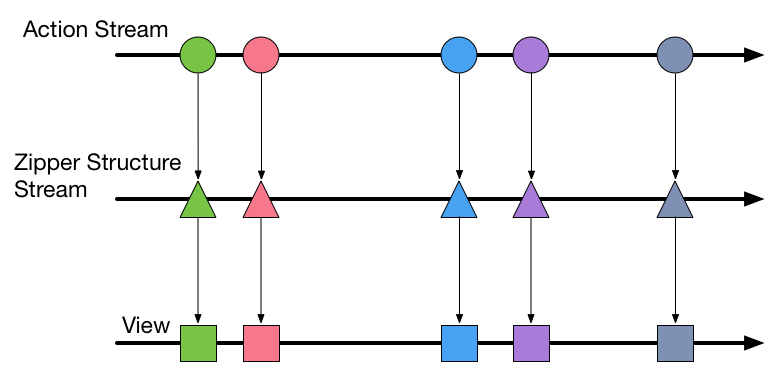
\includegraphics[width=4in]{Implementation_Diagram}
\caption{Implementation Concepts. Each Action,Zipper Structure, View combination is considered to be ``instantaneous''}
\label{fig:FRP}
\end{figure}

The key insight of our implementation strategy is in how to interpret the input from the user.
In a traditional editor, the input from the user is a stream of characters, and there are no guarantees that at any point the program is syntactically correct.
In contrast, in a structured editor, the input from the user is a stream of operations.  These operations can be considered atomic, and will always leave the program in a syntactically correct state.
This insight leads us to conclude that a natural way to implement this editor would be using Functional Reactive Programming~\cite{Wan:2000:FRP:349299.349331} (FRP).
Figure~\ref{fig:FRP} illustrates the concept of an FRP structured editor.
The input from the user is a stream of actions.  Each action results in a change to the underlying model (i.e., a new Zipper Structure object is created after each input action from the user.
Each model change results in an updated view which is then presented to the user.  The user can then consider this new view when they choose a new action as input.

\subsection{HZ}
We explore the concepts presented in the paper in HZ, our current implementation.
In order to reach the widest possible audience, we decided to implement HZ as a web application.
In order to take advantage of all the benefits of FRP, we chose to implement HZ using OCaml\footnote{https://ocaml.org/}, Js\_of\_ocaml\footnote{http://ocsigen.org/js\_of\_ocaml/} and React\footnote{http://erratique.ch/software/react}.
Our code as well as directions for how to run and compile can be found here: \url{https://github.com/MichaelHilton/impl-tfp16}
At the time of submission, HZ should very much be considered a work in progress.

\section{Related Work}
\subsection{Structure Editors}
Drag-and-drop / for novices: lots of examples, e.g. Alice and others

Contemporary: Lamdu, MPS/Mbeddr, TouchDevelop

Hybrid: Cyrus' active code completion paper

%\subsection{Refactoring Models}
%(Michael, can you fill this section out?)

\subsection{Formal Editor Models}
Need to do a search to see what else has been done...

\section{Discussion \& Conclusion}
\subsection{Future Work}
\begin{itemize}
\item More powerful language (codesigned and mechanized as we go along -- having a powerful editor might allow us to dispense with certain complex language features; give example of ad hoc polymorphism?)
\item Keyboard chords
\item Formal action suggestion and ranking models
\item Type-Specific Projections (ala TSLs)
\item Typed Documents
\item Collaboration (packaging system, diff algorithm, multiple cursors, etc.)
\item Connection between our notion of focus in 2.2 and focusing in proof theory
\end{itemize}

This work provides a foundation for studying all of these concepts independently -- show how they work with this system and it should be straightforward to scale to bigger system.

\begin{quote}
In any case, these are but steps toward more graphical program-description systems, for we will not forever stay confined to mere strings of symbols.

--- Minsky, Turing Award lecture
\end{quote}

%
% ---- Bibliography ----
%
% TODO
%\begin{thebibliography}{5}
\bibliographystyle{abbrv}
\bibliography{bibliography}
\end{document}
